\section{三维模型形变技术}
三维模型的形变一直是图形学届所关注的研究课题。
形状建模的早期工作主要聚焦在模型的空间形变,
Barr的工作\cite{barr1984global}就提供了全局的空间重映射。
FFD(Free-form deformation,自由形变)\cite{sederberg1986free}用三维晶格将空间形变参数化,
提供了一个高效的对复杂形状施加粗略形变的方法。
但要得到高质量的形变效果,需要更多细节的控制点\cite{coquillart1990extended},
也会引入更多的手工操作。
常见的网格模型修改工具允许用户移动少量顶点让模型发生形变,同时要保留模型的细节和平滑。
细分和多分辨率技术将网格细节编码为顶点的在拓扑上的
偏移\cite{zorin1997interactive}\cite{kobbelt2000multiresolution}
或者几何上更为简单的基网格\cite{kobbelt1998interactive},
从而在不同的尺度下达到细节保留的目的。
% \begin{figure}[h]
%     \centering
%     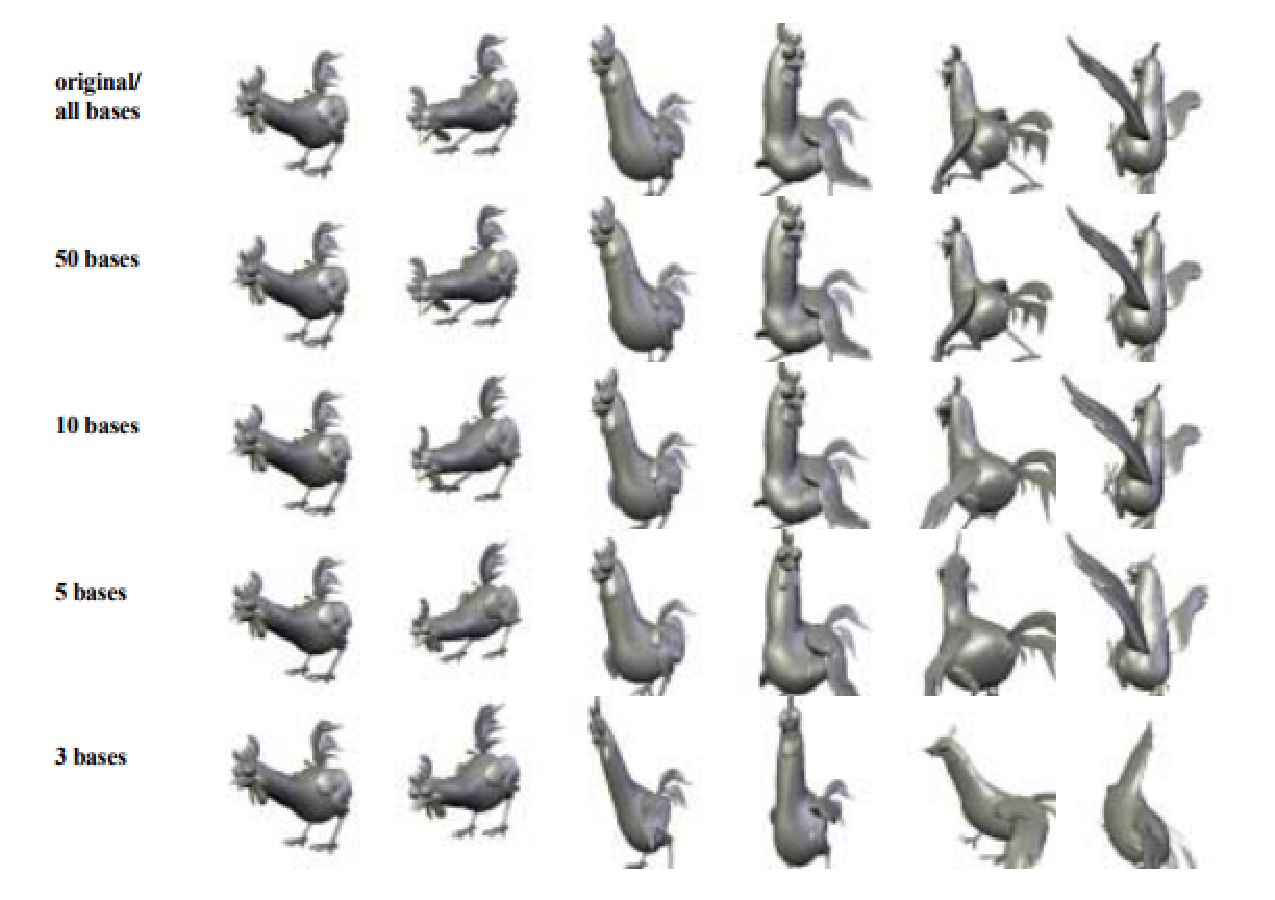
\includegraphics[width=0.95\textwidth]{./Pictures/PCA.eps}
%     \caption{基于PCA的网格动画表示}
%     \label{pca}
% \end{figure}

另一些修改网格的模型的方法则采用了拉普拉斯坐标或金字塔坐标等本征表达。
在这些方法中,每个顶点的位置是由它和相邻节点的关系编码的,
所以局部的改动可以通过本征表达在网格重建的过程中传播的周围的节点。
Yu和Zhou的工作\cite{yu2004mesh}求解了离散在整个网格上的泊松方程。
Sumner提出了形变梯度(deformation-gradient)\cite{sumner2004deformation}来描述形变。
形变梯度描述了三角形网格模型中每一个三角面片相对于参考模型(reference mesh)中对应面片的仿射变换。
Sumner后来提出的Mesh-Based IK\cite{sumner2005mesh}也采用了这种描述形变的方式构建形变子空间,
本文构建子空间采用的也是这一方法。

在三维动画领域,有很多工作致力于基于网格动画序列或集合的压缩表示。
Alexa和Muller\cite{alexa2000representing}用PCA
(Principal Component Analysis,主成分分析)对动画序列。
该方法用一个显现的网格子空间近似表达了网格动画的集合。
相似的,Hauser、Shen和 Brien\cite{hauser2003interactive}
用对弹性方程的模态分析推断所有线性弹性材料的结构共性,
通过对质量和刚度矩阵的特征值分析提取出一组基向量。
该方法易于理解和且实现较为简单但其固有的线性结构导致其不适合描述一些非线性的形变。
比如对于旋转的线性插值会导致网格模型变小。
而且PCA虽然能够很好对已有的网格模型进行压缩,
却不适合构建在主成分所构建的子空间之外的形变。
一些混合式的方法试图解决这一问题,
在某些特殊情况下用骨骼形变描述非线性形变和线性插值相结合\cite{lewis2000pose}。
本文所采用的模型才用了线性插值与非线性插值相结合的方式构建子空间,
对于仿射变换中旋转的部分在李代数上进行插值,对于其他部分则采用线性插值。
